\section{Length-based CM}

LCM resolves conflicts based on the priority of conflicting jobs, besides the length of the interfering atomic section, and the length of the interfered atomic section. This is in contrast to ECM and RCM~\cite{stmconcurrencycontrol:emsoft11}, where conflicts are resolved using the priority of the conflicting jobs. This strategy allows lower priority jobs, under LCM, to retry for lesser time than that under ECM and RCM, but higher priority jobs, sometimes, wait for lower priority ones with bounded priority-inversion.

\subsection{\label{sec 9.1} Design and Rationale}

%Begin algorithm here
\begin{algorithm}
\footnotesize{
\LinesNumbered
\KwData{$s_i^k(\theta)\rightarrow$ interfered atomic section.\\$s_j^l(\theta)\rightarrow$ interfering atomic section.\\$\psi\rightarrow$ predefined threshold $\in [0,1]$.\\$\delta_i^k(\theta)\rightarrow$ remaining execution length of $s_i^k(\theta)$}
\KwResult{which atomic section of $s_i^k(\theta)$ or $s_j^l(\theta)$ aborts}
\eIf{$p_i^k > p_j^l$}
	{$s_j^l(\theta)$ aborts\label{step_sicommits}\;}
	{$c_{ij}^{kl}=len(s_j^l(\theta))/len(s_i^k(\theta))$\label{step_cijkl}\;
	$\alpha_{ij}^{kl}=ln(\psi)/(ln(\psi)-c_{ij}^{kl})$\label{step_alphaijkl}\;
	$\alpha=\left(len(s_i^k(\theta))-\delta_i^k(\theta)\right)/len(s_i^k(\theta))$\;
	\eIf{$\alpha \le \alpha_{ij}^{kl}$}
	{$s_i^k(\theta)$ aborts\label{step_siaborts}\;}
	{$s_j^l(\theta)$ aborts\label{step_sjaborts}\;}
	}
	}
\caption{LCM}
\label{alg_lcm}
\end{algorithm}
%End algorithm here

For both ECM and RCM, $s_{i}^{k}(\theta)$ can be totally repeated if $s_{j}^{l}(\theta)$ --- which belongs to a higher priority job $\tau_{j}^b$ than $\tau_{i}^a$ --- conflicts with $s_{i}^{k}(\theta)$
at the end of its execution, while $s_{i}^{k}(\theta)$ is just about
to commit. Thus, LCM, shown in Algorithm~\ref{alg_lcm}, uses the remaining length of $s_{i}^{k}(\theta)$ when it is interfered,
as well as $len(s_{j}^{l}(\theta))$, to decide which transaction must be aborted. If $p_i^k$ was greater than $p_j^l$, then $s_i^k(\theta)$ would be the one that commits, because it belongs to a higher priority job, and it started before $s_j^l(\theta)$ (step~\ref{step_sicommits}). Otherwise, $c_{ij}^{kl}$ is calculated (step~\ref{step_cijkl}) to determine whether it is worth aborting $s_i^k(\theta)$ in favor of $s_j^l(\theta)$, because $len(s_j^l(\theta))$ is relatively small compared to the remaining execution length of $s_i^k(\theta)$  (explained further).

We assume that:
\begin{equation}
c_{ij}^{kl}=len(s_{j}^{l}(\theta))/len(s_{i}^{k}(\theta))
\label{cm_eq}\end{equation}
where $c_{ij}^{kl}\in]0,\infty[$, to cover all possible lengths of $s_{j}^{l}(\theta)$.
Our idea is to reduce the opportunity for the abort of $s_{i}^{k}(\theta)$ if it is close to committing when interfered and $len(s_{j}^{l}(\theta))$ is large. This abort opportunity is increasingly reduced as $s_{i}^{k}(\theta)$ gets closer to the end of its execution, or $len(s_{j}^{l}(\theta))$ gets larger. 

On the other hand, as $s_{i}^{k}(\theta)$ is interfered early,
or $len(s_{j}^{l}(\theta))$ is small compared to $s_{i}^{k}(\theta)$'s remaining length, the abort opportunity 
is increased even if $s_i^k (\theta)$ is close to the end of its execution. To decide whether $s_{i}^{k}(\theta)$ must be aborted or not, we use a threshold value $\psi\in[0,1]$ that determines $\alpha_{ij}^{kl}$ (step~\ref{step_alphaijkl}), where $\alpha_{ij}^{kl}$ is the maximum percentage of $len(s_i^k(\theta))$ below which $s_j^l(\theta)$ is allowed to abort $s_i^k(\theta)$. Thus, if the already executed part of $s_i^k(\theta)$ --- when $s_j^l(\theta)$ interferes with $s_i^k(\theta)$ --- does not exceed $\alpha_{ij}^{kl}len(s_i^k(\theta))$, then $s_i^k(\theta)$ is aborted (step~\ref{step_siaborts}). Otherwise, $s_j^l(\theta)$ is aborted (step~\ref{step_sjaborts}).

%
\begin{figure}[htbp]
\centering
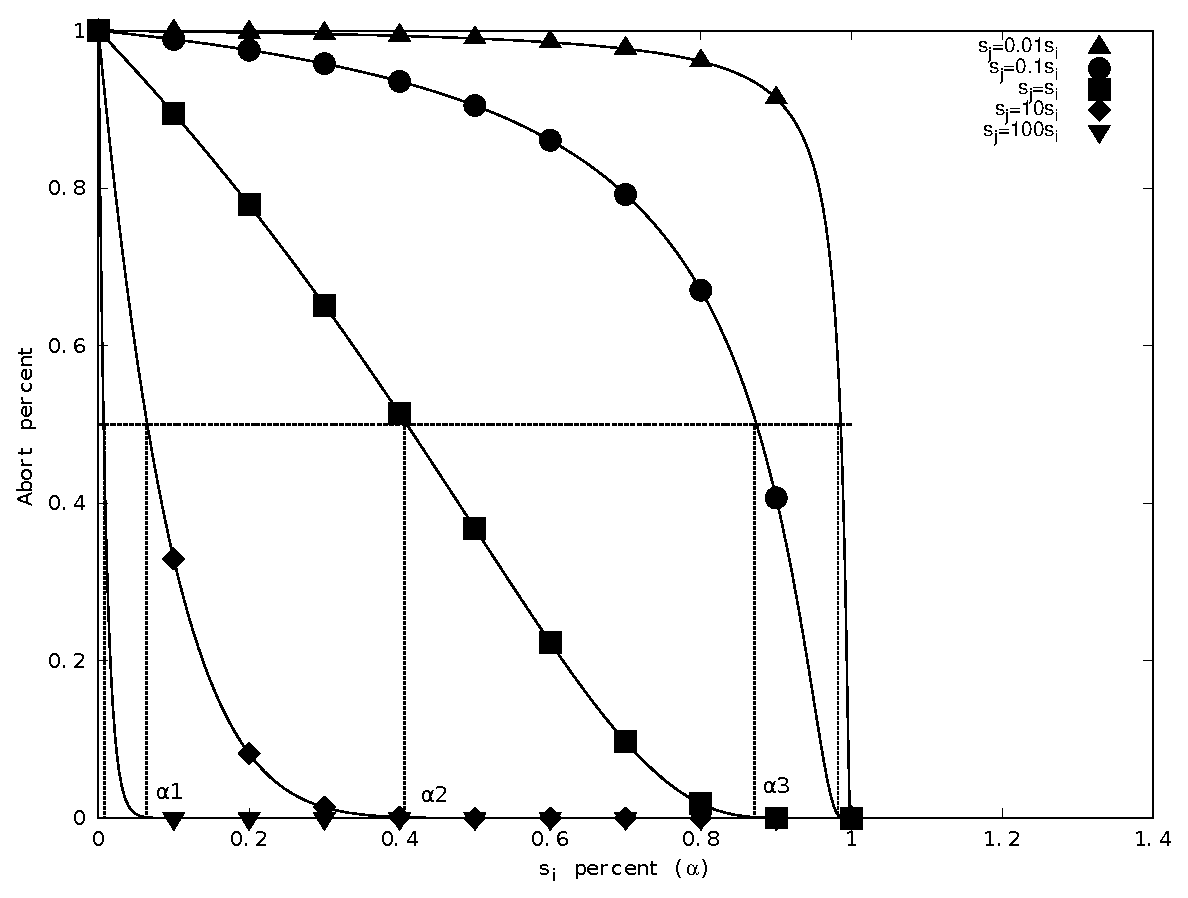
\includegraphics[scale=0.4]{figures/figure16}
\caption{\label{fig16}Interference of $s_{i}^{k}(\theta)$ by various lengths of 
$s_{j}^{l}(\theta)$}
\end{figure}

The behavior of LCM is illustrated in Figure~\ref{fig16}. In this figure, the horizontal axis corresponds to different values of $\alpha$ ranging from $0$ to $1$, and the vertical axis corresponds to different values of abort opportunities, $f(c_{ij}^{kl},\alpha)$, ranging from $0$ to $1$ and calculated by~(\ref{eq49}):
\begin{equation}
f(c_{ij}^{kl},\alpha)=e^{\frac{-c_{ij}^{kl}\alpha}{1-\alpha}}
\label{eq49}\end{equation}
where $c_{ij}^{kl}$ is calculated by~(\ref{cm_eq}).

Figure~\ref{fig16} shows one atomic section $s_i^k(\theta)$ (whose $\alpha$ changes along the horizontal axis) interfered by five different lengths of $s_j^l(\theta)$.
For a predefined value of $f(c_{ij}^{kl},\alpha)$ (denoted as $\psi$ in Algorithm~\ref{alg_lcm}), there corresponds a specific value of $\alpha$ (which is $\alpha_{ij}^{kl}$ in Algorithm~\ref{alg_lcm}) for each curve. For example, when $len(s_j^l(\theta))=0.1 \times len(s_i^k(\theta))$, $s_j^l(\theta)$ aborts $s_i^k(\theta)$ if the latter has not executed more than $\alpha3$ percentage (shown in Figure~\ref{fig16}) of its execution length. As $len(s_{j}^{l}(\theta))$ decreases, the corresponding $\alpha_{ij}^{kl}$ increases (as shown in Figure~\ref{fig16}, $\alpha3>\alpha2>\alpha1$).

Equation (\ref{eq49}) achieves the desired requirement that the abort opportunity is reduced as $s_{i}^{k}(\theta)$ gets
closer to the end of its execution (as $\alpha\rightarrow1,\, f(c_{ij}^{kl},1)\rightarrow0$),
or as the length of the conflicting transaction increases (as $c_{ij}^{kl}\rightarrow\infty,\, f(\infty,\alpha)\rightarrow0$).
Meanwhile, this abort opportunity is increased as $s_{i}^{k}(\theta)$
is interfered closer to its release (as $\alpha\rightarrow0,\, f(c_{ij}^{kl},0)\rightarrow1$),
or as the length of the conflicting transaction decreases (as $c_{ij}^{kl}\rightarrow0,\, f(0,\alpha)\rightarrow1$).

LCM is not a centralized CM, which means that, upon a conflict, each transactions has to decide whether it must commit or abort. 

\begin{clm}
\label{LCM_higher_rc}
Let $s_{j}^{l}(\theta)$ interfere once with $s_{i}^{k}(\theta)$ at $\alpha_{ij}^{kl}$. Then, the maximum contribution of $s_{j}^{l}(\theta)$ to 
$s_{i}^{k}(\theta)$'s 
retry cost is:
\begin{equation}
W_i^k(s_j^l(\theta))\le \alpha_{ij}^{kl}len\Big(s_{i}^{k}(\theta)\Big)+len\Big(s_{j}^{l}(\theta)\Big)\label{eq47}\end{equation}
\end{clm}

\begin{proof}
If $s_{j}^{l}(\theta)$ interferes with $s_{i}^{k}(\theta)$
at a $\Upsilon$ percentage, where $\Upsilon<\alpha_{ij}^{kl}$,
then the retry cost of $s_{i}^{k}(\theta)$ is $\Upsilon len(s_{i}^{k}(\theta))+len(s_{j}^{l}(\theta))$, which is lower than that calculated in (\ref{eq47}). Besides, 
if $s_{j}^{l}(\theta)$ interferes with $s_{i}^{k}(\theta)$ after
$\alpha_{ij}^{kl}$ percentage, then $s_{i}^{k}(\theta)$ will not
abort.
\end{proof}


\begin{clm}
\label{LCM_lower_rc}
An atomic section of a higher priority job, $\tau_{j}^b$, may have to abort and retry due to a lower priority job, $\tau_{i}^a$, if $s_{j}^{l}(\theta)$ interferes
with $s_{i}^{k}(\theta)$ after the $\alpha_{ij}^{kl}$ percentage. $\tau_{j}$'s retry time, due to $s_{i}^{k}(\theta)$ and $s_{j}^{l}(\theta)$,
is upper bounded by:
 \begin{equation}
W_j^l(s_i^k(\theta))\le \Big(1-\alpha_{ij}^{kl}\Big)len\Big(s_{i}^{k}(\theta)\Big)\label{eq48}\end{equation}
\end{clm}

\begin{proof}
It is derived directly from Claim~\ref{LCM_higher_rc}, as $s_j^l(\theta)$ will have to retry for the remaining length of $s_i^k(\theta)$.
\end{proof}

%sh-start
\begin{clm}
\label{no priority inversion in lcm}
Under LCM, there is no priority inversion.
\end{clm}

\begin{proof}
Assume three atomic sections, $s_i^k(\theta)$, $s_j^l(\theta)$, and $s_a^b(\theta)$, where $p_j > p_i$ and $s_j^l(\theta)$ interferes with $s_i^k(\theta)$ after $\alpha_{ij}^{kl}$. Then, $s_j^l(\theta)$ will have to abort and retry. At this time, if $s_a^b(\theta)$ interferes with the other two atomic sections, then LCM decides which transaction to commit by comparing the two transactions. So, we have the following cases:
\begin{itemize}
\item $p_a < p_i < p_j$. Now, $s_a^b(\theta)$ will not abort any one because it is still in its beginning and it is of the lowest priority. Thus, $\tau_j$ is not indirectly blocked by $\tau_a$.
\item $p_i<p_a<p_j$. Now, even if $s_a^b(\theta)$ interferes with $s_i^k(\theta)$ before $\alpha_{ia}^{kb}$,  and $s_a^b(\theta)$ is allowed to abort $s_i^k(\theta)$, after comparing $s_j^l(\theta)$ and $s_a^b(\theta)$, LCM will select $s_j^l(\theta)$ to commit and abort $s_a^b(\theta)$, because the latter is still at its beginning, and $\tau_j$ is of higher priority. If $s_a^b(\theta)$ is not allowed to abort $s_i^k(\theta)$, the situation is still the same, because $s_j^l(\theta)$ was already retrying until $s_i^k(\theta)$ finishes. So, the medium priority instance of $\tau_a$ does not increase the delay time of the higher priority instance of $\tau_j$.
%
\item $p_a>p_j>p_i$. Now, if $s_a^b(\theta)$ is chosen to commit, this will not cause a priority inversion for $\tau_j$ because $\tau_a$ is of higher priority.
\item if $\tau_a$ preempts $\tau_i$, then LCM will compare only between $s_j^l(\theta)$ and $s_a^b(\theta)$. If $p_a<p_j$, then $s_j^l(\theta)$ will commit because of its task's higher priority and $s_a^b(\theta)$ is still at its beginning. Otherwise, $s_j^l(\theta)$ will retry, but this will not be priority inversion, because $\tau_a$ is already of higher priority than $\tau_j$. If $\tau_a$ does not access any object but it preempts $\tau_i$, then LCM will choose $s_j^l(\theta)$ to commit, since only already running transactions are competing together.
\end{itemize}
%
From the previous cases, it appears that priority inversion can never happen under LCM. Claim follows.
\end{proof}

\begin{clm}
\label{priority_inversion}
A higher priority job, $\tau_j^v$, can be delayed by lower priority jobs for at most number of atomic sections in $\tau_j^v$.
\end{clm}

\begin{proof}
By generalizing the cases mentioned in the proof of Claim~\ref{no priority inversion in lcm} to any number of conflicting jobs, it can be seen that when an atomic section, $s_j^l(\theta)$, of a higher priority job conflicts with a number of atomic sections belonging to lower priority jobs, $s_j^l(\theta)$ can be delayed only one of them, $s_i^k(\theta)$, for the remaining length of $s_i^k(\theta)$, then $s_j^l(\theta)$ can run. Thus, the worst case scenario happens when each atomic section in the higher priority job is delayed by one of the atomic sections belonging to lower priority jobs. Claim follows.
\end{proof}
%sh-end


\begin{clm}
\label{max_pri_inv}
The maximum delay suffered by $s_j^l(\theta)$ due to lower priority jobs is caused by the maximum length atomic section accessing object $\theta$, which belongs to a lower priority job than $\tau_j^b$ that owns $s_j^l(\theta)$.
\end{clm}

\begin{proof}
Assume three atomic sections, $s_i^k(\theta)$, $s_j^l(\theta)$, and $s_h^z(\theta)$, where $p_j>p_i$, $p_j>p_h$, and $len(s_i^k(\theta))>len(s_h^z(\theta))$. Now, $\alpha_{ij}^{kl}>\alpha_{hj}^{zl}$ and $c_{ij}^{kl}<c_{hj}^{zl}$. By applying~(\ref{eq48}) to obtain the contribution of $s_i^k(\theta)$ and $s_h^z(\theta)$ to the priority inversion of $s_j^l(\theta)$ and dividing them, we get:
\begin{eqnarray*}
\frac{W_{j}^{l}(s_{i}^{k}(\theta))}{W_{j}^{l}(s_{h}^{z}(\theta))} & = & \frac{\left(1-\alpha_{ij}^{kl}\right)len(s_{i}^{k}(\theta))}{\left(1-\alpha_{hj}^{zl}\right)len(s_{h}^{z}(\theta))}
\end{eqnarray*}
By substitution for $\alpha$s from~(\ref{eq49}):
\begin{eqnarray*}
 & = & \frac{(1-\frac{ln\psi}{ln\psi-c_{ij}^{kl}})len(s_{i}^{k}(\theta))}{(1-\frac{ln\psi}{ln\psi-c_{hj}^{zl}})len(s_{h}^{z}(\theta))}
  =  \frac{(\frac{-c_{ij}^{kl}}{ln\psi-c_{ij}^{kl}})len(s_{i}^{k}(\theta))}{(\frac{-c_{hj}^{zl}}{ln\psi-c_{hj}^{zl}})len(s_{h}^{z}(\theta))}\end{eqnarray*}
$\because ln\psi \le 0$ and $c_{ij}^{kl},c_{hj}^{kl} > 0, \therefore$ by substitution from~(\ref{cm_eq})
\begin{eqnarray*}
 & = & \frac{len(s_{j}^{l}(\theta))/(ln\psi-c_{ij}^{kl})}{len(s_{j}^{l}(\theta))/(ln\psi-c_{hj}^{zl})}
  =  \frac{ln\psi-c_{hj}^{zl}}{ln\psi-c_{ij}^{kl}}>1\end{eqnarray*}
Thus, as the length of the interfered atomic section increases, the delay suffered by the interfering atomic section increases. Claim follows.
\end{proof}


\subsection{\label{response g-edf/lcm} Response Time of G-EDF/LCM}

%Toward establishing the response time under G-EDF/LCM, we introduce a set of Claims.

\begin{clm}\label{GEDF/LCM response time}
$RC(T_i)$ for a task $\tau_i$ under G-EDF/LCM is upper bounded by:
\begin{eqnarray}
RC(T_i) & = & \Bigg(\sum_{\forall \tau_h \in \gamma_i}\sum_{\forall\theta \in \theta_i \wedge \theta_h}\Bigg(\left\lceil\frac{T_{i}}{T_{h}}\right\rceil\sum_{\forall s_{h}^{l}(\theta)}len\Big(s_{h}^{l}(\theta)\Big)\nonumber\\
& + & \alpha_{max}^{hl}len\Big(s_{max}^{h}(\theta)\Big)\Bigg)\Bigg)\nonumber\\
& + & \sum_{\forall s_{i}^{y}(\theta)}\Big(1-\alpha_{max}^{iy}\Big)len\Big(s_{max}^i(\theta)\Big)  
\label{eq78}\end{eqnarray} 
where $\alpha_{max}^{hl}$ is the $\alpha$ value that corresponds to $\psi$ due to the interference of $s_{max}^h(\theta)$ by $s_h^l(\theta)$. $\alpha_{max}^{iy}$ is the $\alpha$ value that corresponds to $\psi$ due to the interference of $s_{max}^i(\theta)$ by $s_i^y(\theta)$.
\end{clm}

\begin{proof}
The maximum number of higher priority instances of $\tau_h$ that can interfere with $\tau_i^x$ is $\left\lceil\frac{T_i}{T_h}\right\rceil$, as shown in Figure~\ref{fig17}, where one instance of $\tau_h$ and $\tau_h^p$ coincides with the absolute deadline of $\tau_i^x$.

By using Claims~\ref{LCM_higher_rc},~\ref{LCM_lower_rc},~\ref{priority_inversion}, and~\ref{max_pri_inv}, and Claim 1 in~\cite{stmconcurrencycontrol:emsoft11} to determine the effect of atomic sections belonging to higher and lower priority instances of interfering tasks to $\tau_i^x$, Claim follows.
\end{proof}


Response time of $\tau_{i}$ is calculated by (11) in~\cite{stmconcurrencycontrol:emsoft11}.
\begin{figure}
\begin{centering}
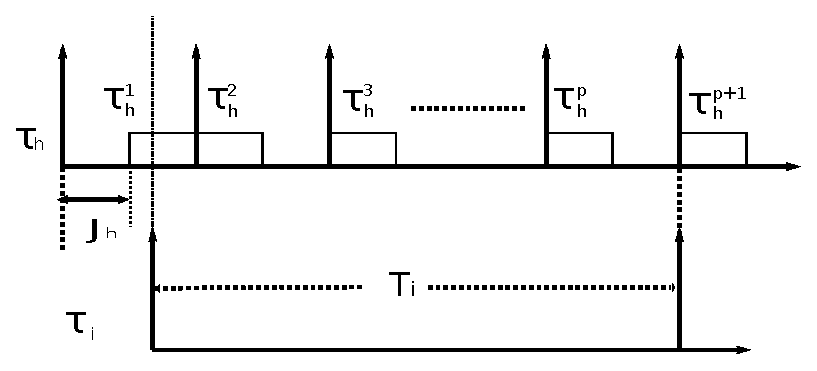
\includegraphics[scale=0.6]{figures/figure18}
\par\end{centering}
\caption{\label{fig17}$\tau_h^p$ has a higher priority than $\tau_i^x$}
\end{figure}

\subsection{Schedulability of G-EDF/LCM and ECM}
\label{performance g-edf-lcm}
We now compare the schedulability of G-EDF/LCM with ECM~\cite{stmconcurrencycontrol:emsoft11} %(FMLP and OMLPprotocols~\cite{key-4,brandenburg2008comparison,key-3}), 
to understand when G-EDF/LCM will perform better. 
Toward this, we compare the total utilization of ECM with that of G-EDF/LCM. For each method, we inflate the $c_i$ of each task $\tau_i$ by adding the retry cost suffered by $\tau_i$. Thus, if method $A$ adds retry cost $RC_A(T_i)$ to $c_i$, and method $B$ adds retry cost $RC_B(T_i)$ to $c_i$, then the schedulability of $A$ and $B$ are compared as:
\begin{eqnarray}
\sum_{\forall \tau_{i}}\frac{c_{i}+RC_A(T_{i})}{T_{i}} & \le & \sum_{\forall \tau_{i}}\frac{c_{i}+RC_B(T_{i})}{T_{i}}\nonumber\\
\sum_{\forall \tau_{i}}\frac{RC_A(T_{i})}{T_{i}} & \le & \sum_{\forall \tau_{i}}\frac{RC_B(T_{i})}{T_{i}}
\label{eqa}\end{eqnarray}
Thus, schedulability is compared by substituting the retry cost added by the synchronization methods in (\ref{eqa}).

\begin{clm}\label{lcm versus ecm}
Let $s_{max}$ be the maximum length atomic section accessing any object $\theta$. Let $\alpha_{max}$ and $\alpha_{min}$ be the maximum and minimum values of $\alpha$ for any two atomic sections $s_i^k(\theta)$ and $s_j^l(\theta)$. Given a threshold $\psi$, schedulability of G-EDF/LCM is equal or better than ECM if for any task $\tau_i$:
\begin{equation}
\frac{1-\alpha_{min}}{1-\alpha_{max}} \le \sum_{\forall \tau_h \in \gamma_i}\left\lceil\frac{T_i}{T_h}\right\rceil
\label{edf-lcm-ecm}\end{equation}
\end{clm}

\begin{proof}
Under ECM, $RC(T_{i})$ is upper bounded by:
\begin{equation}
RC(T_{i})\le\sum_{\forall \tau_{h}\in\gamma_{i}}\sum_{\forall \theta\in\ (\theta_{i}\wedge\theta_{h})}\left(\left\lceil\frac{T_{i}}{T_{h}}\right\rceil\sum_{\forall s_{h}^{z}(\theta)}2len(s_{max})\right)\label{eq61}\end{equation}
with the assumption that all lengths of atomic sections of (4) and (8) in~\cite{stmconcurrencycontrol:emsoft11} and~(\ref{eq78}) are replaced by $s_{max}$.
%~\cite{stmconcurrencycontrol:emsoft11}. 
Let $\alpha_{max}^{hl}$ in~(\ref{eq78}) be replaced with $\alpha_{max}$, and $\alpha_{max}^{iy}$ in~(\ref{eq78}) be replaced with $\alpha_{min}$. 
As $\alpha_{max}$, $\alpha_{min}$, and $len(s_{max})$ are all constants, (\ref{eq78}) is upper bounded by:
\begin{eqnarray}
RC(T_i) & \le & \Bigg(\sum_{\forall \tau_h \in \gamma_i}\sum_{\forall\theta \in \theta_i \wedge \theta_h}\Bigg(\left\lceil\frac{T_{i}}{T_{h}}\right\rceil\sum_{\forall s_{h}^{l}(\theta)}\left(1+\alpha_{max}\right)\nonumber\\
& & len\Big(s_{max}\Big)\Bigg)\Bigg)
 +  \sum_{\forall s_{i}^{y}(\theta)}\Big(1-\alpha_{min}\Big)len\Big(s_{max}\Big)\nonumber\\ 
\label{eq101}\end{eqnarray}
%
If $\beta_1^{ih}$ is the total number of times any instance of $\tau_h$ accesses shared objects with $\tau_i$, then $\beta_1^{ih}=\sum_{\forall \theta\in(\theta_{i}\wedge\theta_{h})}\sum_{\forall s_{h}^{z}(\theta)}$. Furthermore, if $\beta_2^i$ is the total number of times any instance of $\tau_i$ accesses shared objects with any other instance,   $\beta_2^i=\sum_{\forall s_{i}^{y}(\theta)}$\textit{, where $\theta$ is shared with another task}. Then, $\beta_{i}=max\{max_{\forall \tau_h \in \gamma_i}\{\beta_1^{ih}\},\beta_2^i\}$ is the maximum number of accesses to all shared objects by any instance of $\tau_{i}$ or $\tau_{h}$. 
Thus, (\ref{eq61}) becomes:
\begin{equation}
RC(T_{i})\le\sum_{\tau_{h}\in\gamma_{i}}2\left\lceil\frac{T_{i}}{T_{h}}\right\rceil\beta_{i}len(s_{max})
\label{eq63}\end{equation}
and (\ref{eq101}) becomes:
\begin{eqnarray}
RC(T_{i}) & \le & \beta_{i}len(s_{max}) \Bigg((1-\alpha_{min})\nonumber\\
& + & \sum_{\forall \tau_h \in \gamma_i}\left\lceil\frac{T_{i}}{T_{h}}\right\rceil(1+\alpha_{max})\Bigg)
\label{eq102}\end{eqnarray}

We can now compare the total utilization of G-EDF/LCM with that of ECM by comparing~(\ref{eq101}) and~(\ref{eq102}) for all $\tau_i$:
\begin{eqnarray}
& & \sum_{\forall \tau_{i}}\frac{(1-\alpha_{min})+\sum_{\forall \tau_{h}\in\gamma_{i}}\left(\left\lceil\frac{T_{i}}{T_{h}}\right\rceil(1+\alpha_{max})\right)}{T_{i}} \nonumber\\
& \le &   \sum_{\forall \tau_{i}}\frac{\sum_{\forall \tau_{h}\in\gamma_{i}}2\left\lceil\frac{T_{i}}{T_{h}}\right\rceil}{T_{i}}\label{eqc}\end{eqnarray}

(\ref{eqc}) is satisfied if for each $\tau_{i}$, the following condition is satisfied:
\begin{equation*}
(1-\alpha_{min})+\sum_{\forall \tau_h \in \gamma_i}\left(\left\lceil\frac{T_{i}}{T_{h}}\right\rceil(1+\alpha_{max})\right)  \le  2\sum_{\forall \tau_h \in \gamma_i}\left\lceil\frac{T_{i}}{T_{h}}\right\rceil
\end{equation*}
\begin{equation*}
\therefore\frac{1-\alpha_{min}}{1-\alpha_{max}}  \le  \sum_{\forall \tau_h \in \gamma_i}\left\lceil\frac{T_{i}}{T_{h}}\right\rceil
\end{equation*}
Claim follows.
\end{proof}


\subsection{G-EDF/LCM versus Lock-free}
\label{gedf-lcm-lock-free}
We consider the retry-loop lock-free synchronization for G-EDF given in~\cite{key-5}. This lock-free approach is the most relevant to our work. 

\begin{clm}\label{gedf-lcm-lock-free_clm} 
Let $s_{max}$ denote $len(s_{max})$ and $r_{max}$ denote the maximum execution cost of a single iteration of any retry loop of any task in the retry-loop lock-free algorithm in~\cite{key-5}. Now, G-EDF/LCM achieves higher schedulability than the retry-loop lock-free approach if the upper bound on $s_{max}/r_{max}$ under G-EDF/LCM ranges between 0.5 and 2 (which is higher than that under  ECM). 
\end{clm}

\begin{proof}
From~\cite{key-5}, the retry-loop lock-free algorithm
is upper bounded by: 
\begin{equation}
RL(T_{i})=\sum_{\tau_{h}\in\gamma_{i}}\left(\left\lceil \frac{T_{i}}{T_{h}}\right\rceil +1\right)\beta_{i}r_{max}\label{eq32_1}
\end{equation}
 where $\beta_{i}$ is as defined in Claim~\ref{lcm versus ecm}.
The retry cost of $\tau_{i}$ in G-EDF/LCM is upper bounded by (\ref{eq102}).
By comparing G-EDF/LCM's total utilization with that of the retry-loop
lock-free algorithm, we get: 
\begin{eqnarray*}
 & \sum_{\forall\tau_{i}}\frac{\left((1-\alpha_{min})+\sum_{\forall\tau_{h}\in\gamma_{i}}\left(\left\lceil \frac{T_{i}}{T_{h}}\right\rceil (1+\alpha_{max})\right)\right)\beta_{i}s_{max}}{T_{i}}\\
\le & \sum_{\forall\tau_{i}}\frac{\sum_{\forall\tau_{h}\in\gamma_{i}}\left(\left\lceil \frac{T_{i}}{T_{h}}\right\rceil +1\right)\beta_{i}r_{max}}{T_{i}}
\end{eqnarray*}
 
\begin{eqnarray}
\therefore\frac{s_{max}}{r_{max}}\le\frac{\sum_{\forall\tau_{i}}\frac{\sum_{\forall\tau_{h}\in\gamma_{i}}\left(\left\lceil \frac{T_{i}}{T_{h}}\right\rceil +1\right)\beta_{i}}{T_{i}}}{\sum_{\forall\tau_{i}}\frac{\left((1-\alpha_{min})+\sum_{\forall\tau_{h}\in\gamma_{i}}\left(\left\lceil \frac{T_{i}}{T_{h}}\right\rceil (1+\alpha_{max})\right)\right)\beta_{i}}{T_{i}}}\label{u-gedf-lcm-ecm}
\end{eqnarray}


Let the number of tasks that have shared objects with $\tau_{i}$
be $\omega$ (i.e., $\sum_{\tau_{h}\in\gamma_{i}}=\omega\ge1$ since
at least one task has a shared object with $\tau_{i}$; otherwise,
there is no conflict between tasks). Let the total number of tasks
be $n$, so $1\le\omega\le n-1$, and $\left\lceil \frac{T_{i}}{T_{h}}\right\rceil \in[1,\infty[$.
To find the minimum and maximum values for the upper bound on $s_{max}/r_{max}$,
we consider the following cases: 
\begin{itemize}
\item $\alpha_{min}\rightarrow0,\alpha_{max}\rightarrow0$ 
\end{itemize}
$\therefore$~(\ref{u-gedf-lcm-ecm}) will be: 
\begin{eqnarray}
\frac{s_{max}}{r_{max}} & \le & 1+\frac{\sum_{\forall\tau_{i}}\frac{\omega-1}{T_{i}}}{\sum_{\forall\tau_{i}}\frac{1+\sum_{\forall\tau_{h}\in\gamma_{i}}\left\lceil \frac{T_{i}}{T_{h}}\right\rceil }{T_{i}}}\nonumber \\
\label{s-r-1}
\end{eqnarray}
 By substituting the edge values for $\omega$ and $\left\lceil \frac{T_{i}}{T_{h}}\right\rceil $
in~(\ref{s-r-1}), we derive that the upper bound on $s_{max}/r_{max}$
lies between 1 and 2.
\begin{itemize}
\item $\alpha_{min}\rightarrow0,\alpha_{max}\rightarrow1$ 
\end{itemize}
(\ref{u-gedf-lcm-ecm}) becomes 
\begin{eqnarray}
\frac{s_{max}}{r_{max}} & \le & 0.5+\frac{\sum_{\forall\tau_{i}}\frac{\omega-0.5}{T_{i}}}{\sum_{\forall\tau_{i}}\frac{1+2\sum_{\forall\tau_{h}\in\gamma_{i}}\left\lceil \frac{T_{i}}{T_{h}}\right\rceil }{T_{i}}}\label{s-r-2}
\end{eqnarray}
 By applying the edge values for $\omega$ and $\left\lceil \frac{T_{i}}{T_{h}}\right\rceil $
in~(\ref{s-r-2}), we derive that the upper bound on $s_{max}/r_{max}$
lies between 0.5 and 1.
\begin{itemize}
\item $\alpha_{min}\rightarrow1,\alpha_{max}\rightarrow0$ 
\end{itemize}
This case is rejected since $\alpha_{min}\le\alpha_{max}$.
\begin{itemize}
\item $\alpha_{min}\rightarrow1,\alpha_{max}\rightarrow1$ 
\end{itemize}
$\therefore$~(\ref{u-gedf-lcm-ecm}) becomes: 
\begin{eqnarray}
\frac{s_{max}}{r_{max}} & \le & 0.5+\frac{\sum_{\tau_{i}}\frac{\omega}{T_{i}}}{2\sum_{\tau_{i}}\frac{\sum_{\forall\tau_{h}\in\gamma_{i}}\left\lceil \frac{T_{i}}{T_{h}}\right\rceil }{T_{i}}}\label{s-r-4}
\end{eqnarray}
 By applying the edge values for $\omega$ and $\left\lceil \frac{T_{i}}{T_{h}}\right\rceil $
in~(\ref{s-r-4}), we derive that the upper bound on $s_{max}/r_{max}$
lies between 0.5 and 1, which is similar to that achieved by ECM.

Summarizing from the previous cases, the upper bound on $s_{max}/r_{max}$
lies between 0.5 and 2, whereas for ECM~\cite{stmconcurrencycontrol:emsoft11},
it lies between 0.5 and 1. Claim follows.

\end{proof}

\subsection{Response Time of G-RMA/LCM}
\label{rma}

\begin{clm}\label{response g-rma/lcm}
Let $\lambda_{2}(j,\theta)=\sum_{\forall s_{j}^{l}(\theta)}len(s_{j}^{l}(\theta))+\alpha_{max}^{jl}len(s_{max}^{j}(\theta))$, where $\alpha_{max}^{jl}$ is the $\alpha$ value corresponding to $\psi$ due to the interference of $s_{max}^j(\theta)$ by $s_j^l(\theta)$. The retry cost of any task $\tau_i$ under G-RMA/LCM during $T_i$ 
is given by:
\begin{eqnarray}
RC\left(T_i\right) & = &
  \sum_{\forall \tau_{j}^{*}}\left(\sum_{\theta\in(\theta_{i}\wedge\theta_{j})}\left(\left(\left\lceil\frac{T_i}{T_{j}}\right\rceil +1\right)\lambda_{2}(j,\theta)\right)\right)\nonumber\\
& + & \sum_{\forall s_{i}^{y}(\theta)}\Big(1-\alpha_{max}^{iy}\Big)len\Big(s_{max}^i(\theta)\Big)
\label{eq60}
\end{eqnarray}
where $\tau_{j}^{*}=\{\tau_{j}|(\tau_{j}\in\gamma_{i})\wedge(p_{j}>p_{i})\}$.
\end{clm}

\begin{proof}
Under G-RMA, all instances of a higher priority task, $\tau_{j}$, can conflict with a lower priority task,
$\tau_{i}$, during $T_{i}$. (\ref{eq47}) can be used to determine the contribution of each conflicting atomic section in $\tau_j$ to $\tau_i$. Meanwhile, all instances of any task with lower priority than $\tau_{i}$ can conflict with $\tau_i$ during $T_{i}$. Claims~\ref{LCM_lower_rc} and~\ref{priority_inversion} can be used to determine the contribution of conflicting atomic sections in lower priority tasks to $\tau_i$.
%
  %over the whole $t(T_i)$ (unlike the case of G-EDF/LCM, where (\ref{eq59}) chooses which equation to use depending on whether or not $L$ is less than $\left\lfloor\frac{t(T_{i})-c_{h}}{t(T_{h})}\right\rfloor t(T_{h})+c_{h}$).
Using the previous notations and Claim 3 in~\cite{stmconcurrencycontrol:emsoft11}, the Claim follows.
\end{proof}

The response time is calculated by (17) in~\cite{stmconcurrencycontrol:emsoft11} with replacing $RC(R_i^{up})$ with $RC(T_i)$.
%BR: You should say "..with $RC(T_i)$ replacing $RC(R_i^{up})$."

\subsection{Schedulability of G-RMA/LCM and RCM}
\label{rma eval}

\begin{clm}\label{rma_eval_clm}
Under the same assumptions of Claims~\ref{lcm versus ecm} and~\ref{response g-rma/lcm}, G-RMA/LCM's schedulability is equal or better than RCM if:
\begin{equation}
\frac{1-\alpha_{min}}{1-\alpha_{max}}\le \sum_{\forall \tau_j^*}\left( \left\lceil\frac{T_i}{T_j}\right\rceil +1 \right)
\label{eq70}\end{equation}
\end{clm}

\begin{proof}
Under the same assumptions as that of Claims~\ref{lcm versus ecm} and~\ref{response g-rma/lcm}, (\ref{eq60}) can be upper bounded as:
\begin{eqnarray}
RC(T_i) & \le & \sum_{\forall \tau_{j}^{*}}\bigg(\left(\left\lceil\frac{T_{i}}{T_{j}}\right\rceil +1\right)(1+\alpha_{max})
 len(s_{max})\beta_{i}\bigg)\nonumber\\
 & + & (1-\alpha_{min})len(s_{max})\beta_{i}\label{eq68}\end{eqnarray}
 
For RCM, (16) in~\cite{stmconcurrencycontrol:emsoft11} for $RC(T_{i})$ is upper bounded by:
\begin{equation*}
RC(T_{i})\le\sum_{\forall \tau_{j}^{*}}\left(\left\lceil\frac{T_{i}}{T_{j}}\right\rceil +1\right)2\beta_{i}len(s_{max})\label{eq69}\end{equation*}\
By comparing the total utilization of G-RMA/LCM with that of RCM,
we get:
\begin{eqnarray}
 & \sum_{\forall\tau_{i}}\frac{len\left(s_{max}\right)\beta_{i}\left(\left(1-\alpha_{min}\right)+\sum_{\forall\tau_{j}^{*}}\left(\left(\left\lceil\frac{T_{i}}{T_{j}}\right\rceil+1\right)\left(1+\alpha_{max}\right)\right)\right)}{T_{i}}\nonumber\\
\le & \sum_{\forall\tau_{i}}\frac{2len\left(s_{max}\right)\beta_{i}\sum_{\forall\tau_{j}^{*}}\left(\left\lceil\frac{T_{i}}{T_{j}}\right\rceil+1\right)}{T_{i}}\label{grma-lcm-rcm}\end{eqnarray}
(\ref{grma-lcm-rcm}) is satisfied if $\forall \tau_i$~(\ref{eq70}) is satisfied. Claim follows.
\end{proof}

%NEWNEW-start
\subsection{G-RMA/LCM versus Lock-free}\label{g-rma lcm vs lock-free}

Although~\cite{key-5} considers retry-loop lock-free synchronization
for G-EDF systems,~\cite{key-5} also applies for G-RMA systems.

\begin{clm}\label{lcm rma lock-free comparison clm}

Let $s_{max}$ denote $len(s_{max})$ and $r_{max}$ denote the maximum
execution cost of a single iteration of any retry loop of any task
in the retry-loop lock-free algorithm in~\cite{key-5}. G-RMA/LCM
achieves higher schedulability than the retry-loop lock-free approach
if the upper bound on $s_{max}/r_{max}$ under G-RMA/LCM is no less
than 0.5. Upper bound on $s_{max}/r_{max}$ can extend to large values
when $\alpha_{min}$ and $\alpha_{max}$ are very large.

\end{clm}

\begin{proof}

Retry cost for G-RMA/LCM is upper bounded by~(\ref{eq60}). Let $\gamma_{i}=\tau_{j}^{*}\cup\bar{\tau_{j}}$,
where $\tau_{j}^{*}$ is the set of higher priority tasks than $\tau_{i}$
sharing objects with $\tau_{i}$. $\bar{\tau_{j}}$ is the set
of lower priority tasks than $\tau_{i}$ sharing objects with
it. We follow the same definitions of $\beta_{i},\, r_{max}$ and
$RL(T_{i})$ given in the proof of Claim (\ref{gedf-lcm-lock-free_clm}).
Schedulability of G-RMA/LCM equals or exceeds schedulability of retry-loop
lock-free if 

\begin{eqnarray}
\frac{s_{max}}{r_{max}} & \le & \frac{\sum_{\forall\tau_{i}}\frac{\sum_{\tau_{j}^{*}}\left(\left\lceil \frac{T_{i}}{T_{j}}\right\rceil +1\right)}{T_{i}}}{\sum_{\forall\tau_{i}}\frac{\Big(1-\alpha_{min}\Big)+\sum_{\tau_{j}^{*}}\left(\left\lceil \frac{T_{i}}{T_{j}}\right\rceil +1\right)\left(1+\alpha_{max}\right)}{T_{i}}}\nonumber\\
 & + & \frac{2\sum_{\forall\tau_{i}}\frac{\sum_{\forall\bar{\tau_{j}}}}{T_{i}}}{\sum_{\forall\tau_{i}}\frac{\Big(1-\alpha_{min}\Big)+\sum_{\tau_{j}^{*}}\left(\left\lceil \frac{T_{i}}{T_{j}}\right\rceil +1\right)\left(1+\alpha_{max}\right)}{T_{i}}}\nonumber\\
 & & \label{eq:lcm rma lock-free comparison 1} 
\end{eqnarray}


If $p_{j}<p_{i},\,\therefore\,\left\lceil \frac{T_{i}}{T_{j}}\right\rceil =1$
because the system assumes impilicit deadline tasks and uses G-RMA
scheduler. 
%
Let $\omega_{1}$ be size of $\tau_i^*$ and $\omega_{2}$
be size of $\bar{\tau_i}$. $\therefore$ $\omega_{1}^{i}\ge 1$ and $\omega_{2}^{i}\ge1$.
Otherwise, there is no conflict with $\tau_{i}$. To find the maximum
and minimum upper bounds for $s_{max}/r_{max}$, the following cases
are considered:
\begin{itemize}
\item $\alpha_{min}\rightarrow0,\,\alpha_{max}\rightarrow0$


\begin{equation}
\therefore\frac{s_{max}}{r_{max}}\le1+\frac{\sum_{\forall\tau_{i}}\frac{2\omega_{2}^{i}-1}{T_{i}}}{\sum_{\forall\tau_{i}}\frac{1+\sum_{\tau_{j}^{*}}\left(\left\lceil \frac{T_{i}}{T_{j}}\right\rceil +1\right)}{T_{i}}}\label{eq:lcm rma lock-free comparison 3}
\end{equation}
As the second term in (\ref{eq:lcm rma lock-free comparison 3}) is
alawys positive (because $\omega_{2}^{i}\ge1$), then the minimum
upper bound on $s_{max}/r_{max}$ is $1$. To get the maximum upper
bound on $s_{max}/r_{max}$, let $\left\lceil \frac{T_{i}}{T_{j}}\right\rceil $
approaches its minimum value $1$, $\omega_{1}^{i}\rightarrow0,\,\omega_{2}^{i}\rightarrow n-1$ (the
maximum and minimum values for $\omega_{1}^{i}$ and $\omega_{2}^{i}$
respectively. $n$ is number of tasks), then 
\[
\therefore\frac{s_{max}}{r_{max}}\le\left(2n-2\right)
\]
Of course, $n$ cannot be lower than $2$. Otherwise, there will be
no conflicting tasks.

\item $\alpha_{min}\rightarrow0,\,\alpha_{max}\rightarrow1$


\begin{equation}
\frac{s_{max}}{r_{max}}\le\frac{1}{2}+\frac{\sum_{\forall\tau_{i}}\frac{4\omega_{2}^{i}-1}{T_{i}}}{2\sum_{\forall\tau_{i}}\frac{1+2\sum_{\tau_{j}^{*}}\left(\left\lceil \frac{T_{i}}{T_{j}}\right\rceil +1\right)}{T_{i}}}\label{eq:lcm rma lock-free comparison 4}
\end{equation}
The minimum upper bound for $s_{max}/r_{max}$ is $0.5$. This can
happen when $T_{i}\gg T_{j}$. To get the maximum upper bound on $s_{max}/r_{max}$,
let $\left\lceil \frac{T_{i}}{T_{j}}\right\rceil $ approaches its
minimum value $1$, $\omega_{2}^{i}\rightarrow n-1,\,\omega_{1}^{i}\rightarrow0$,
then 
\[
\frac{s_{max}}{r_{max}}\le2n-2
\]


\item $\alpha_{min}\rightarrow1,\,\alpha_{max}\rightarrow0$


This case is rejected because $\alpha_{max}$ must be greater or equal
to $\alpha_{min}$.

\item $\alpha_{min}\rightarrow1,\,\alpha_{max}\rightarrow1$


\begin{equation}
\frac{s_{max}}{r_{max}}\le\frac{1}{2}+\frac{\sum_{\forall\tau_{i}}\frac{\omega_{2}^{i}}{T_{i}}}{\sum_{\forall\tau_{i}}\frac{\sum_{\tau_{j}^{*}}\left(\left\lceil \frac{T_{i}}{T_{j}}\right\rceil +1\right)}{T_{i}}}\label{eq:lcm rma lock-free comparison 5}
\end{equation}
The minimum upper bound for $s_{max}/r_{max}$ is $0.5$. This can
happen when $T_{i}\gg T_{j}$. To get the maximum upper bound on $s_{max}/r_{max}$,
let $\left\lceil \frac{T_{i}}{T_{j}}\right\rceil $ approaches its
minimum value $1$, $\omega_{2}^{i}\rightarrow n-1,\,\omega_{1}^{i}\rightarrow0$,
then 
\[
\frac{s_{max}}{r_{max}}\rightarrow\infty
\]


\end{itemize}
From the previous cases, we can derive that upper bound on $s_{max}/r_{max}$
extends from $0.5$ to large values. Claim follows.

\end{proof}
%NEWNEW-end

\section{Experimental Evaluation}\label{exp_eval}

Having established LCM's retry and response time upper bounds, and the conditions under which it outperforms ECM, RCM, and lock-free synchronization, we now would like to understand how LCM's retry and response times in practice (i.e., on average) compare with that of competitor methods. Since this can only be understood experimentally, we implement LCM and the competitor methods and conduct experimental studies. 

\subsection{Experimental Setup}
We used the ChronOS real-time Linux kernel~\cite{dellinger2011chronos}
and the RSTM library~\cite{marathe2006lowering}. We modified RSTM to include implementations of ECM, RCM, G-EDF/LCM, and G-RMA/LCM contention managers, and modified ChronOS to include implementations of G-EDF and G-RMA schedulers. 

For the retry-loop lock-free implementation,
we used a loop that reads an object and attempts to write to the object using a compare-and-swap (CAS) instruction. The task retries until the CAS succeeds. 
%We call this lock-free operation, CAS-loop operation.

We use an 8 core, 2GHz AMD Opteron platform. The average time
taken for one write operation by RSTM on any
core is 0.0129653375$\mu s$, and the average time taken
by one CAS-loop operation on any core is 0.0292546250 $\mu s$.

We used the periodic task set shown in Table~\ref{tab:Task-set-1}. Each task runs in its own thread and has a set of atomic sections. Atomic section properties are probabilistically controlled (for experimental evaluation) using three parameters: the maximum and minimum lengths of any atomic section within the task, and the total length of atomic sections within any task. All task atomic sections access the same object, and do write operations on the object (thus, contention is the highest).

\begin{table}
\caption{\label{tab:Task-set-1}Task sets. (a) \label{tab:Task-sets-(a)} Task set 1: 5-task set; 
\label{tab:Task-sets-(b)} (b) Task set 2: 10-task set; \label{tab:Task-sets-(c)} (c) Task set 3: 12-task set}
\centering{}\begin{tabular}{|c|c|c|}
\multicolumn{3}{c}{(a)}\tabularnewline
\cline{2-3} 
\multicolumn{1}{c|}{} & $T_{i}(\mu s)$ & $c_{i}(\mu s)$\tabularnewline
\hline 
$\tau_{1}$ & 500000 & 150000\tabularnewline
\hline 
$\tau_{2}$ & 1000000 & 227000\tabularnewline
\hline 
$\tau_{3}$ & 1500000 & 410000\tabularnewline
\hline 
$\tau_{4}$ & 3000000 & 299000\tabularnewline
\hline 
$\tau_{5}$ & 5000000 & 500000\tabularnewline
\hline
\end{tabular} \begin{tabular}{|c|c|c|}
\multicolumn{3}{c}{(b)}\tabularnewline
\cline{2-3} 
\multicolumn{1}{c|}{} & $T_{i}(\mu s)$ & $c_{i}(\mu s)$\tabularnewline
\hline 
$\tau_{1}$ & 400000 & 75241\tabularnewline
\hline 
$\tau_{2}$ & 750000 & 69762\tabularnewline
\hline 
$\tau_{3}$ & 1200000 & 267122\tabularnewline
\hline 
$\tau_{4}$ & 1500000 & 69863\tabularnewline
\hline 
$\tau_{5}$ & 2400000 & 152014\tabularnewline
\hline 
$\tau_{6}$ & 4000000 & 286301\tabularnewline
\hline 
$\tau_{7}$ & 7500000 & 493150\tabularnewline
\hline 
$\tau_{8}$ & 10000000 & 794520\tabularnewline
\hline 
$\tau_{9}$ & 15000000 & 1212328\tabularnewline
\hline 
$\tau_{10}$ & 20000000 & 1775342\tabularnewline
\hline
\end{tabular} \begin{tabular}{|c|c|c|}
\multicolumn{3}{c}{(c)}\tabularnewline
\cline{2-3} 
\multicolumn{1}{c|}{} & $T_{i}(\mu s)$ & $c_{i}(\mu s)$\tabularnewline
\hline 
$\tau_{1}$ & 400000 & 58195\tabularnewline
\hline 
$\tau_{2}$ & 750000 & 53963\tabularnewline
\hline 
$\tau_{3}$ & 1000000 & 206330\tabularnewline
\hline 
$\tau_{4}$ & 1200000 & 53968\tabularnewline
\hline 
$\tau_{5}$ & 1500000 & 117449\tabularnewline
\hline 
$\tau_{6}$ & 2400000 & 221143\tabularnewline
\hline 
$\tau_{7}$ & 3000000 & 290428\tabularnewline
\hline 
$\tau_{8}$ & 4000000 & 83420\tabularnewline
\hline 
$\tau_{9}$ & 7500000 & 380917\tabularnewline
\hline 
$\tau_{10}$ & 10000000 & 613700\tabularnewline
\hline 
$\tau_{11}$ & 15000000 & 936422\tabularnewline
\hline 
$\tau_{12}$ & 20000000 & 1371302\tabularnewline
\hline
\end{tabular}
\end{table}

\subsection{Results}

Figure \ref{fig:RC_results} shows the retry cost (RC) 
for each task in the three task sets in Table \ref{tab:Task-set-1}, where each task has a single atomic section of length equal to 0.2 of the task length. Each data point in the figure has a confidence level of 0.95. We observe that G-EDF/LCM and G-RMA/LCM achieve shorter
or comparable retry cost than ECM and RCM. Since all tasks are initially
released at the same time, and due to the specific nature of task properties, tasks with lower IDs somehow have higher priorities under the G-EDF scheduler. Note that tasks with lower IDs have higher priorities under G-RMA, since tasks are ordered in non-decreasing order of their periods. 

Thus, we observe that G-EDF/LCM and G-RMA/LCM achieve comparable retry costs
to ECM and RCM for some tasks with lower IDs. But when task ID increases,
LCM --- for both schedulers --- achieves much shorter retry costs 
than ECM and RCM. 
This is because, higher priority tasks in LCM can be delayed by lower priority tasks, which is not the case for ECM and RCM. However, as task priority decreases, LCM, by definition, prevents higher priority
tasks from aborting lower priority ones if a higher priority task
interferes with a lower priority one after a specified threshold. In contrast, under ECM and RCM, lower priority tasks abort in favor of higher priority ones. G-EDF/LCM and G-RMA/LCM also achieve shorter retry costs than the retry-loop lock-free algorithm.

\begin{figure}[htbp]
\centering
\subfigure[Task set 1]{
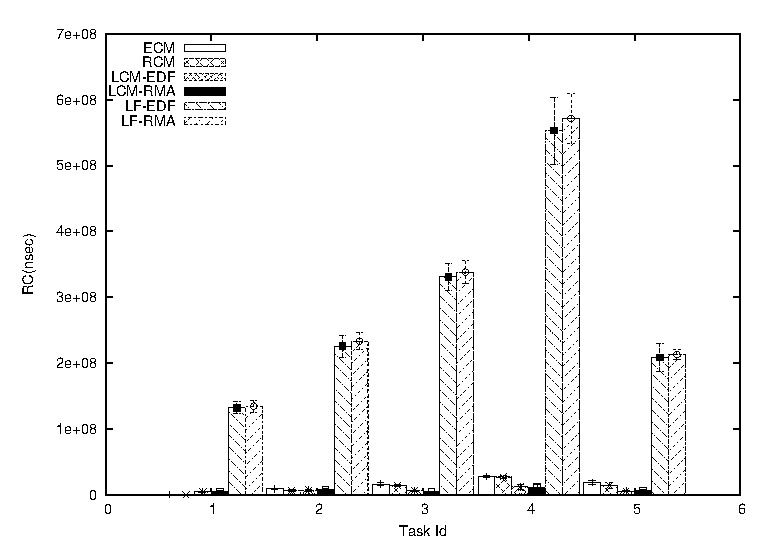
\includegraphics[scale=0.6]
{figures/Abr_dur_5t_nl_g_30_0.2_0.2_0.2_1.eps}
\label{fig-RC-set1}
}
\subfigure[Task set 2]{
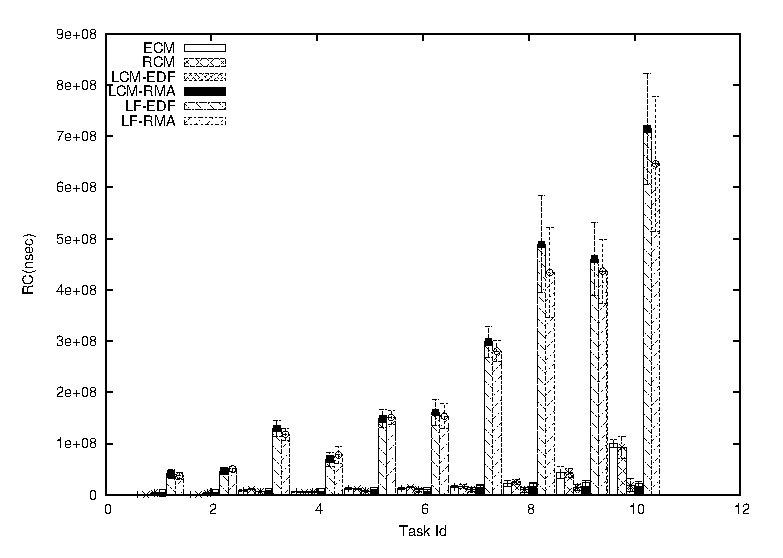
\includegraphics[scale=0.6]{figures/Abr_dur_10t_nl_g_30_0.2_0.2_0.2_1.eps}
\label{fig-RC-set2}
}
\subfigure[Task set 3]{
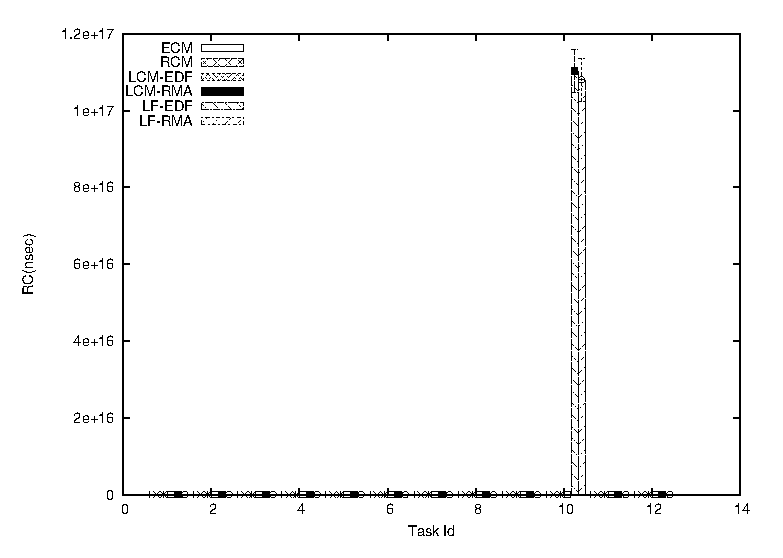
\includegraphics[scale=0.6]{figures/Abr_dur_12t_nl_g_30_0.2_0.2_0.2_1.eps}
\label{fig-RC-set3}
}
\caption{Task retry costs under LCM and competitor synchronization methods}
\label{fig:RC_results}
\end{figure}

Figure \ref{fig:res_results-1} shows the response time of each task of the task sets in Table \ref{tab:Task-set-1} with a confidence level of 0.95. (Again, each task's atomic section length is equal to half of the task length.) 
We observe that G-EDF/LCM and G-RMA/LCM achieve shorter 
response time than the retry-loop lock-free
algorithm, and shorter 
or comparable response time than ECM and RCM.

\begin{figure}[htbp]
\subfigure[Task set 1]{
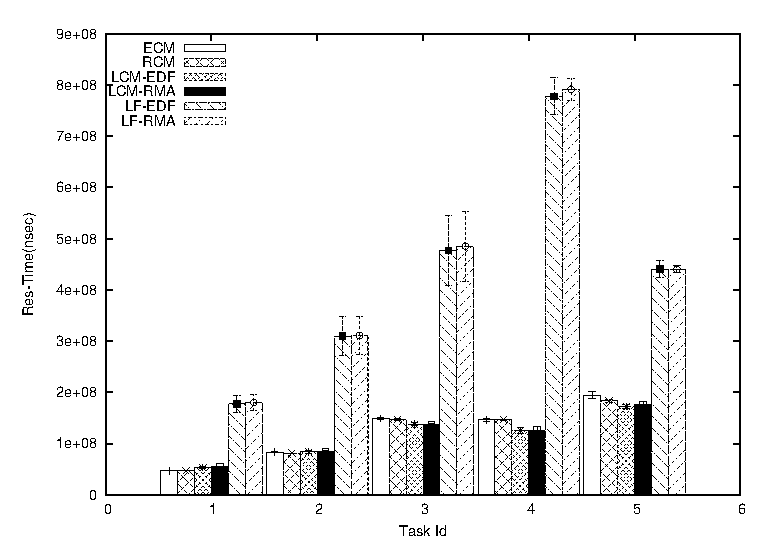
\includegraphics[scale=0.6]{figures/Res_Time_5t_nl_g_30_0.2_0.2_0.2_1.eps}
\label{fig-res-set1-1}
}
\subfigure[Task set 2]{
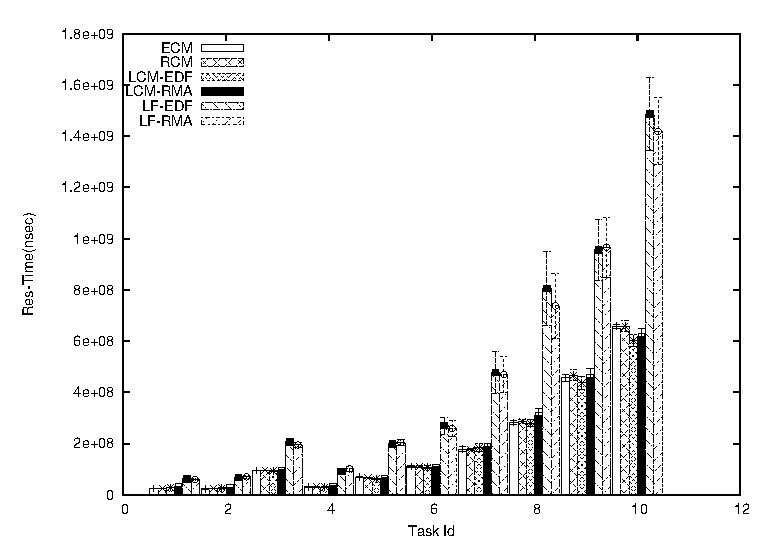
\includegraphics[scale=0.6]{figures/Res_Time_10t_nl_g_30_0.2_0.2_0.2_1.eps}
\label{fig-res-set2-1}
}
\subfigure[Task set 3 ]{
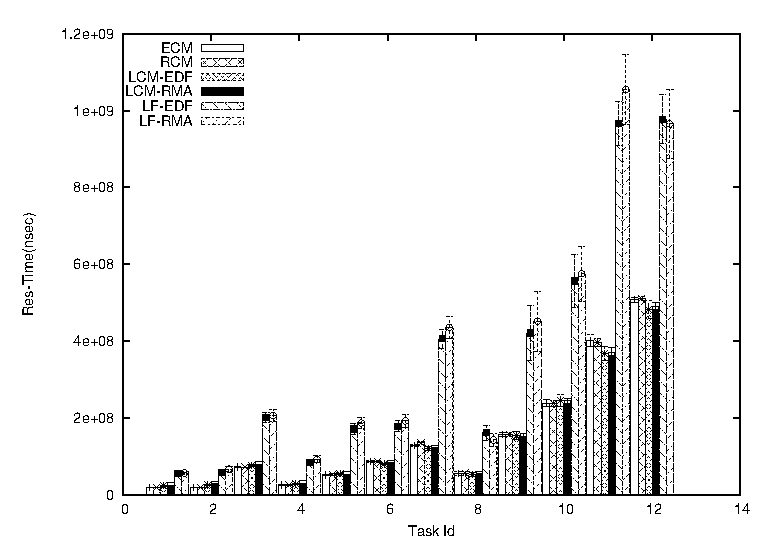
\includegraphics[scale=0.6]{figures/Res_Time_12t_nl_g_30_0.2_0.2_0.2_1.eps}
\label{fig-res-set3-1}
}
\caption{Task response times under LCM and competitor synchronization methods}
\label{fig:res_results-1}
\end{figure}

We repeated the experiments by varying the number and length of atomic sections. Due to space limitation, only subset of results are shown in Figures~\ref{fig:RC_results 5 2 2} to~\ref{fig:res_results 8 5 2}. 
%NEWNEW-start
A complete set of results are shown in Appendix B in~\cite{stmconcurrencycontrol_techreport}. Each figure has three parameters $x,y,z$ in the lable. $x$ specifies the relative total length of all atomic sections to the length of the task. $y$ specifies the maximum relative length of any atomic section to the length of the task. $z$ specifies the minimum relative length of any atomic section to the length of the task. These figures show a consistent trend with previous results.
%NEWNEW-end

\begin{figure}[htbp]
\centering
\subfigure[Task set 1]{
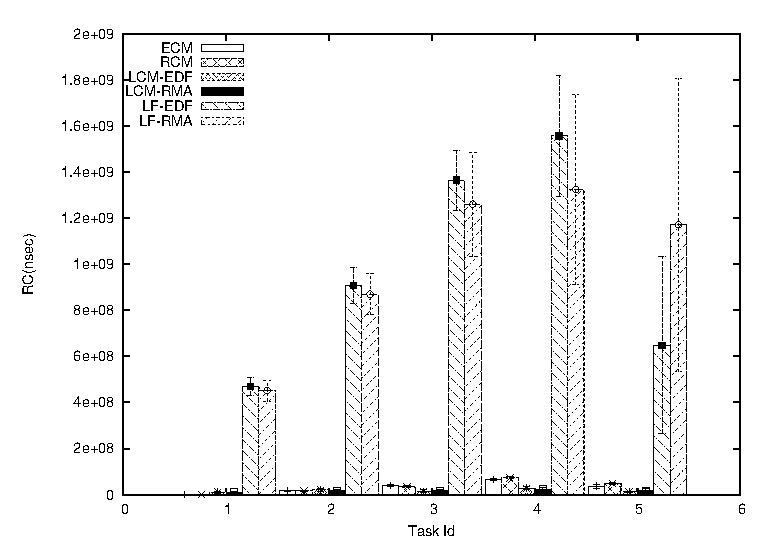
\includegraphics[scale=0.6]
{figures/Abr_dur_5t_nl_g_30_0.5_0.2_0.2_1.eps}
\label{fig-RC-set1}
}
\subfigure[Task set 2]{
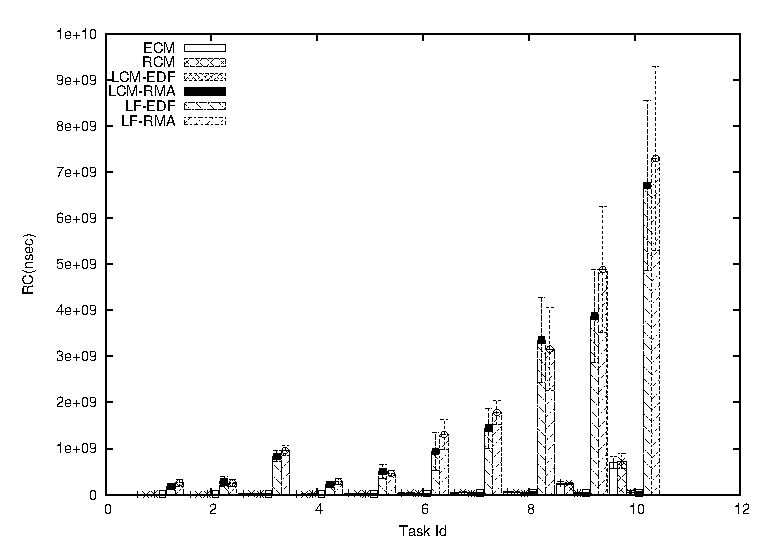
\includegraphics[scale=0.6]{figures/Abr_dur_10t_nl_g_30_0.5_0.2_0.2_1.eps}
\label{fig-RC-set2}
}
\subfigure[Task set 3]{
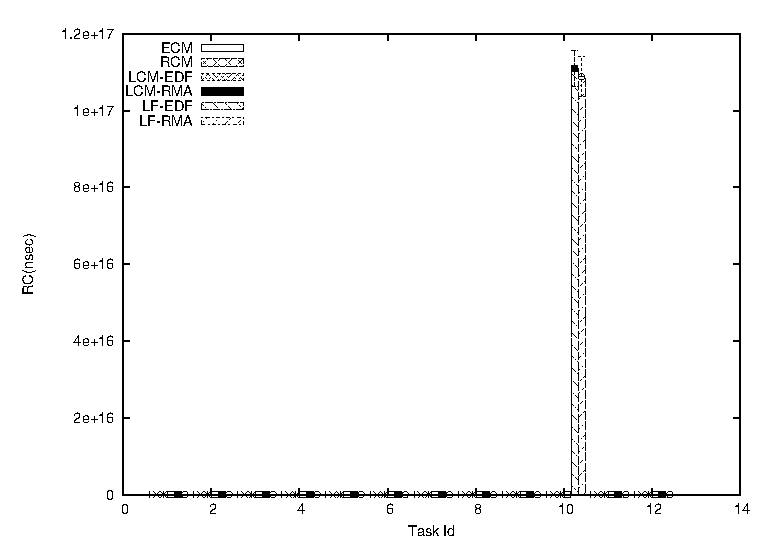
\includegraphics[scale=0.6]{figures/Abr_dur_12t_nl_g_30_0.5_0.2_0.2_1.eps}
\label{fig-RC-set3}
}
\caption{Task retry costs under LCM and competitor synchronization methods (0.5,0.2,0.2)}
\label{fig:RC_results 5 2 2}
\end{figure}

\begin{figure}[htbp]
\subfigure[Task set 1]{
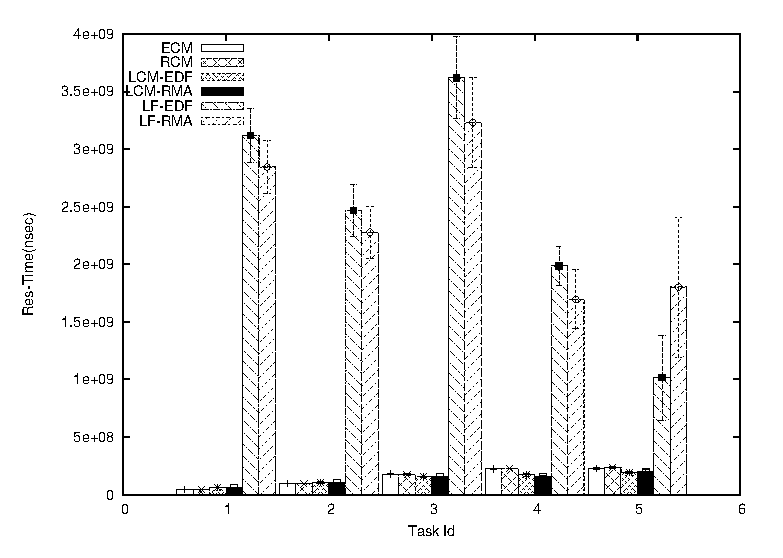
\includegraphics[scale=0.6]{figures/Res_Time_5t_nl_g_30_0.5_0.2_0.2_1.eps}
\label{fig-res-set1-1}
}
\subfigure[Task set 2]{
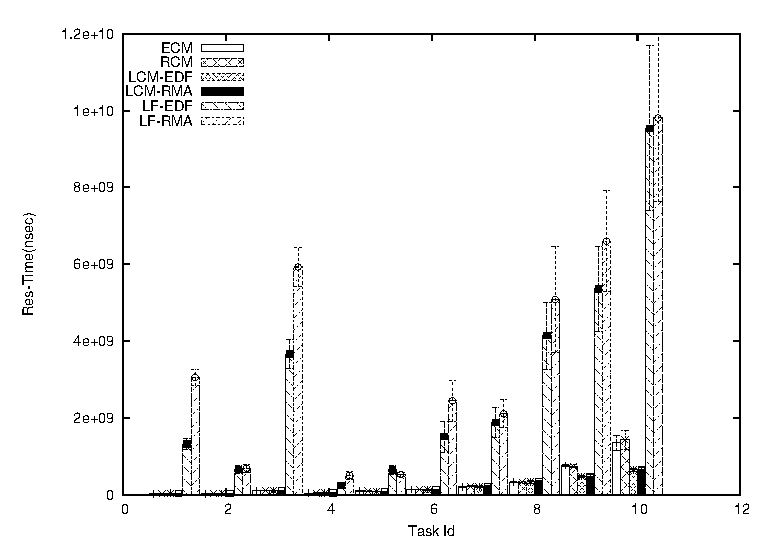
\includegraphics[scale=0.6]{figures/Res_Time_10t_nl_g_30_0.5_0.2_0.2_1.eps}
\label{fig-res-set2-1}
}
\subfigure[Task set 3 ]{
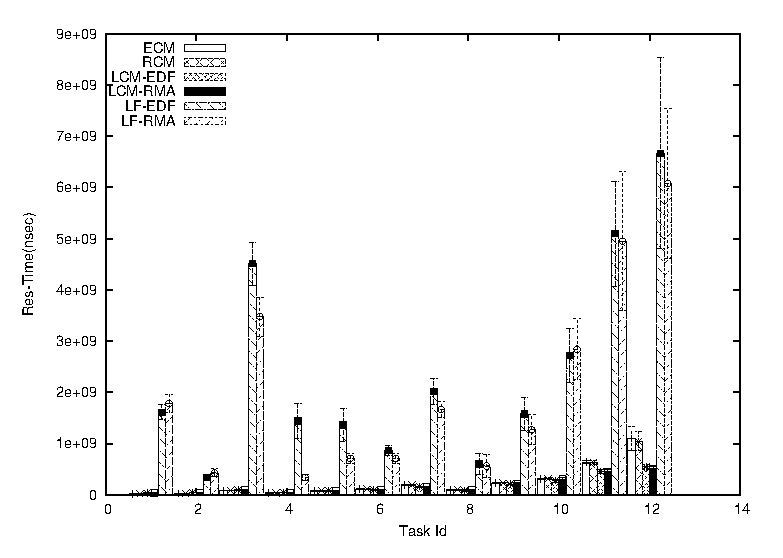
\includegraphics[scale=0.6]{figures/Res_Time_12t_nl_g_30_0.5_0.2_0.2_1.eps}
\label{fig-res-set3-1}
}
\caption{Task response times under LCM and competitor synchronization methods (0.5,0.2,0.2)}
\label{fig:res_results 5 2 2}
\end{figure}

\begin{figure}[htbp]
\centering
\subfigure[Task set 1]{
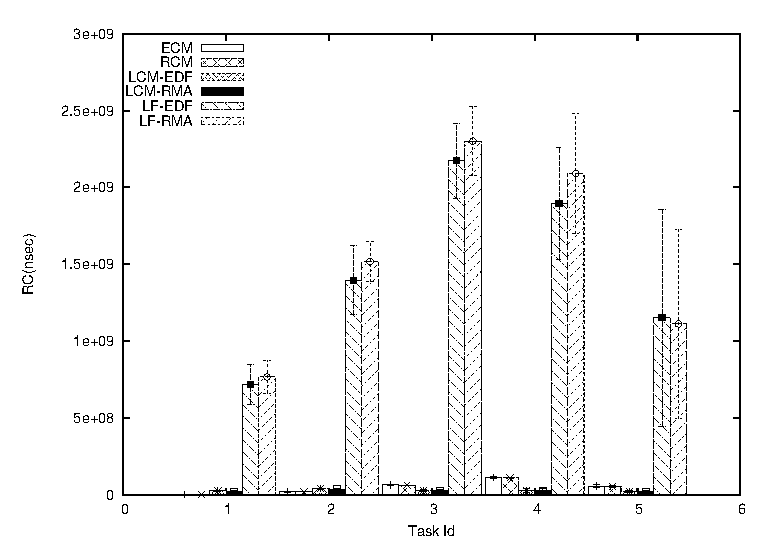
\includegraphics[scale=0.6]
{figures/Abr_dur_5t_nl_g_30_0.8_0.5_0.2_1.eps}
\label{fig-RC-set1}
}
\subfigure[Task set 2]{
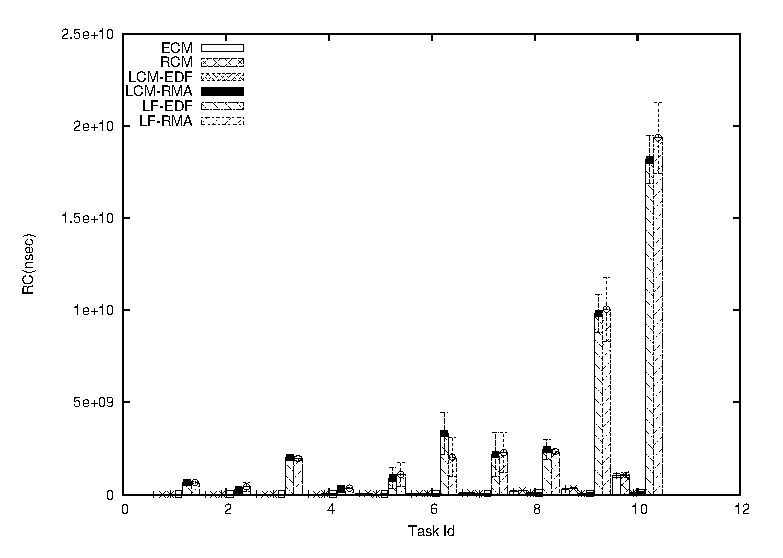
\includegraphics[scale=0.6]{figures/Abr_dur_10t_nl_g_30_0.8_0.5_0.2_1.eps}
\label{fig-RC-set2}
}
\subfigure[Task set 3]{
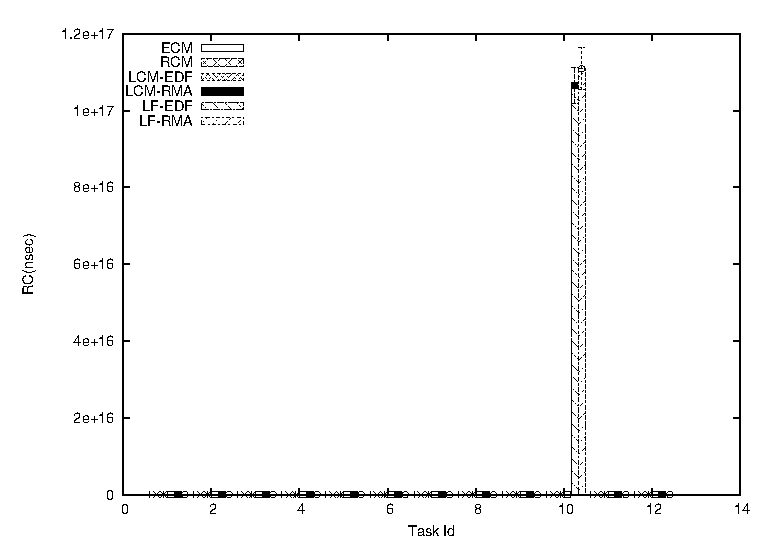
\includegraphics[scale=0.6]{figures/Abr_dur_12t_nl_g_30_0.8_0.5_0.2_1.eps}
\label{fig-RC-set3}
}
\caption{Task retry costs under LCM and competitor synchronization methods (0.8,0.5,0.2)}
\label{fig:RC_results 8 5 2}
\end{figure}

\begin{figure}[htbp]
\subfigure[Task set 1]{
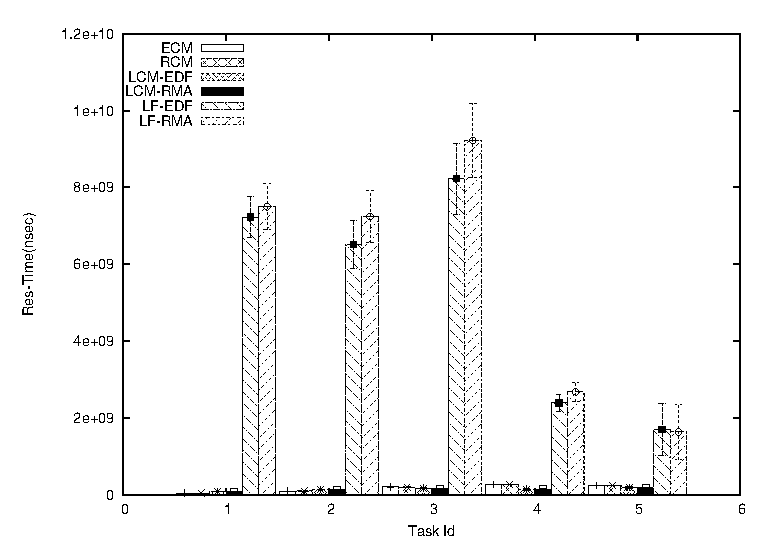
\includegraphics[scale=0.6]{figures/Res_Time_5t_nl_g_30_0.8_0.5_0.2_1.eps}
\label{fig-res-set1-1}
}
\subfigure[Task set 2]{
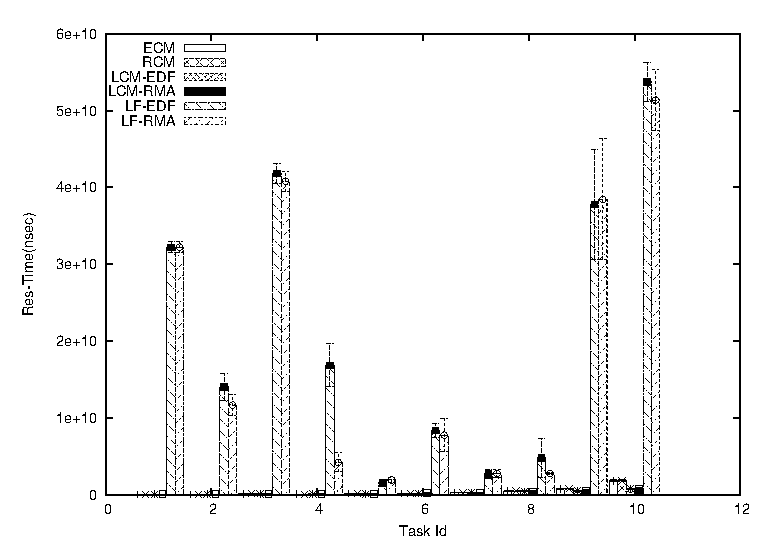
\includegraphics[scale=0.6]{figures/Res_Time_10t_nl_g_30_0.8_0.5_0.2_1.eps}
\label{fig-res-set2-1}
}
\subfigure[Task set 3 ]{
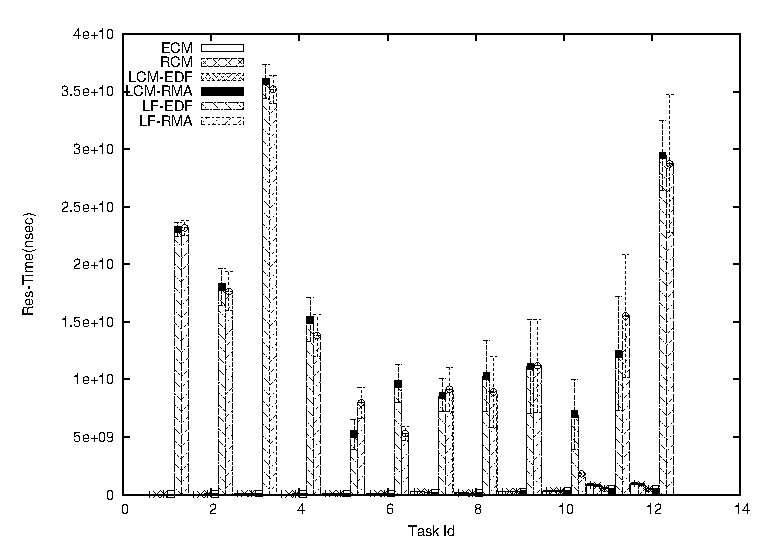
\includegraphics[scale=0.6]{figures/Res_Time_12t_nl_g_30_0.8_0.5_0.2_1.eps}
\label{fig-res-set3-1}
}
\caption{Task response times under LCM and competitor synchronization methods (0.8,0.5,0.2)}
\label{fig:res_results 8 5 2}
\end{figure}



\section{Conclusions}
\label{sec:conclusions_lcm}

In ECM and RCM, a task incurs at most $2s_{max}$ retry cost for each of its atomic section due to conflict
with another task's atomic section. With LCM, this retry cost is reduced to $(1+\alpha_{max})s_{max}$ for each aborted atomic section. In ECM and RCM, tasks do not retry due to lower priority tasks, whereas in LCM, they do so. In G-EDF/LCM, retry due to a lower priority job is encountered only from a task $\tau_{j}$'s last job instance 
during $\tau_{i}$'s period. This is not the case with G-RMA/LCM, because,  each higher priority task can be aborted and retried by any job instance of lower priority tasks. Schedulability of G-EDF/LCM and G-RMA/LCM is better or equal to ECM and RCM, respectively, by proper choices for $\alpha_{min}$ and $\alpha_{max}$. Schedulability of G-EDF/LCM is better than retry-loop lock-free synchronization for G-EDF if the upper bound on $s_{max}/r_{max}$ is between 0.5 and 2, which is higher than that achieved by ECM. 
%sh-new-start
G-RMA/LCM acheives higher schedulability than retry-loop lock-free if $s_{max}/r_{max}$ is not less than 0.5. For high values of $\alpha$ in G-RMA/LCM, $s_{max}/r_{max}$ can extend to large values.
%sh-new-end
